% !TeX document-id = {2870843d-1baa-4f6a-bd0a-a5c796104a32}
% !BIB TS-program = biber
% !TeX encoding = UTF-8
% TU Delft beamer template

\documentclass[aspectratio=43]{beamer}
\usepackage[english]{babel}
\usepackage{csquotes}
\usepackage{calc}
\usepackage[absolute,overlay]{textpos}
\usepackage{graphicx}
\usepackage{subfig}
\usepackage{mathtools}
\usepackage{amsfonts}
\usepackage{amsthm}
\usepackage{comment}
\usepackage{siunitx}
\usepackage{MnSymbol,wasysym}
\usepackage{array}
\usepackage{qrcode}
\useoutertheme[subsection=false]{miniframes}

\setbeamertemplate{navigation symbols}{} % remove navigation symbols
\mode<presentation>{\usetheme[verticalbar=false]{tud}}

% BIB SETTINGS
\usepackage[
    backend=biber,
    giveninits=true,
    maxnames=30,
    maxcitenames=20,
    uniquename=init,
    url=false,
    style=authoryear,
]{biblatex}
\addbibresource{bibfile.bib}
\setlength\bibitemsep{0.3cm} % space between entries in the reference list
\renewcommand{\bibfont}{\normalfont\scriptsize}
\setbeamerfont{footnote}{size=\tiny}
\renewcommand{\cite}[1]{\footnote<.->[frame]{\fullcite{#1}}}
\setlength{\TPHorizModule}{\paperwidth}
\setlength{\TPVertModule}{\paperheight}

\newcommand{\absimage}[4][0.5,0.5]{%
	\begin{textblock}{#3}%width
		[#1]% alignment anchor within image (centered by default)
		(#2)% position on the page (origin is top left)
		\includegraphics[width=#3\paperwidth]{#4}%
\end{textblock}}

\newcommand{\mininomen}[2][1]{{\let\thefootnote\relax%
	\footnotetext{\begin{tabular}{*{#1}{@{\!}>{\centering\arraybackslash}p{1em}@{\;}p{\textwidth/#1-2em}}}%
	#2\end{tabular}}}}

\title[]{Localización de landmarks cefalométricos por medio de técnicas de few-shot learning y análisis de redes convolucionales}
\institute[]{\textbf{Tutores}: Pablo Mesejo Santiago, Javier Merí de la Maza \and Universidad de Granada, España}
\author{Alejandro Borrego Megías}
\date{\today}



%%%%%%%%%%%%% EMPIEZA LA PRESENTACION %%%%%%%%%%%%%
\begin{document}

{
\setbeamertemplate{footline}{\usebeamertemplate*{minimal footline}}
\frame{\titlepage}
}

% Parte de Matemáticas
\part{Análisis de Redes convolucionales}

%INDICE
\begin{frame}{Índice Primera Parte}
  \textcolor{tudCyan}{\textbf{Análisis de redes convolucionales}}
  \medskip
  \tableofcontents[part=1]
\end{frame}

% DIAPOSITIVA ANTES DE CADA SECCION
\AtBeginSection[ ]
{
\begin{frame}{Índice Primera Parte}
    \tableofcontents[currentsection]
\end{frame}
}

%INTRODUCCION
\section{Introducción}
  \begin{frame}[fragile]{Redes Neuronales Convolucionales}
    \begin{itemize}
      \item Buen rendimiento, comprobable empíricamente.
      \item Vía de estudio abierta en lo que se refiere a
      la modelización matemática y la justificación teórica de estos resultados.
    \end{itemize}

    Destacamos: 

    \begin{figure}
      \centering
      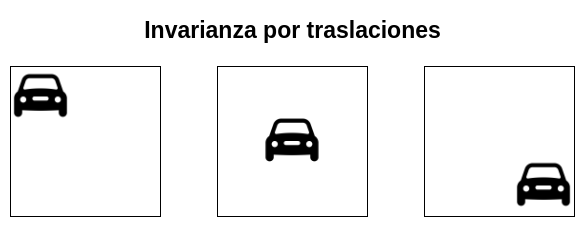
\includegraphics[width=0.4\textwidth]{imgs/translation_invariance.png}
    \end{figure}

    \begin{figure}
      \centering
      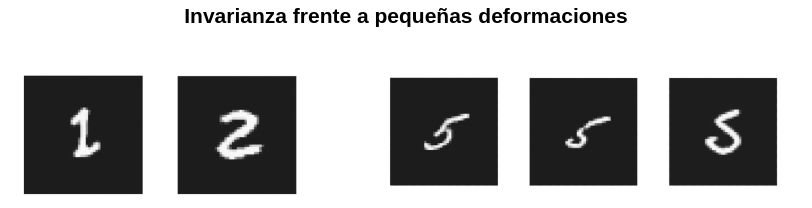
\includegraphics[width=0.7\textwidth]{imgs/Deformaciones.png}
    \end{figure}
  \end{frame}

  \begin{frame}{Invarianza por traslaciones}
    Trabajamos sobre el espacio de funciones $L^2(\mathbb{R}^d)$.

    \begin{block}{Definición de traslación}
       Sea $f\in L^2(\mathbb{R}^d)$, $L_cf(x)=f(x-c)$ es la traslación de $f$ por $c \in \mathbb{R}^d$.
    \end{block}

    \begin{block}{Invarianza por traslaciones de un operador $\Phi$}
      Decimos que un operador $\Phi$ sobre  $L^2(\mathbb{R}^d)$, es invariante por traslaciones si $\Phi(L_cf(x))=\Phi(f)$ para todo $f \in L^2(\mathbb{R}^d)$ y para todo $c \in \mathbb{R}^d$.
   \end{block}
  \end{frame}

  \begin{frame}{Invarianza frente a pequeñas deformaciones}
    \textcolor{tudCyan}{\textit{Deformación $\implies$ Difeomorfismo}}

    \textcolor{tudCyan}{\textit{Deformaciones pequeñas $\implies$ Difeomorfismo cercanos a traslaciones}}  

    \begin{block}{Definición}
      Denotemos $L_{\tau} f(x)=f(x-\tau(x))$ como la acción del difeomorfismo $1-\tau$ sobre $f$.

      Donde $\tau$ es el campo de desplazamiento. 
    \end{block}

    \textcolor{tudCyan}{\textbf{\centering Invarianza frente a pequeñas deformaciones \\ \centering $\Downarrow$ \\ \centering Lipschitz-continuidad frente a la acción de difeomorfismos}}  
  \end{frame}

  \begin{frame}{Invarianza frente a pequeñas deformaciones}

    \begin{block}{Condición de Lipschitz clásica}
      Sea $f: M \rightarrow N$ una función entre dos espacios métricos $M$ y $N$ con sus respectivas distancias $d_M$ y $d_N$. Se dice que $f$ satisface la condición de Lipschitz si $\exists C>0$ tal que: 
      $$d_N(f(x),f(y))\leq C d_M(x,y), \; \; \forall x,y \in M$$ 
    \end{block}

    En nuestro caso: 

    \begin{equation}
      \|\Phi(f) - \Phi(L_\tau f) \| \leq \|f\| · d(1, 1-\tau)
    \end{equation}

    Necesitamos una definición para la distancia entre dichos difeomorfismos.
  \end{frame}


  \begin{frame}{Invarianza frente a pequeñas deformaciones}
    \begin{block}{Distancia entre $1-\tau$ y $1$}
      Se define una distancia entre $1-\tau$ y $1$ en cualquier subconjunto compacto $\Omega$ de $\mathbb{R}^d$ como 
      \begin{equation} \label{eq::distancia}
        d_\Omega(1,1-\tau) = \sup_{x \in \Omega} |\tau (x)| + \sup_{x \in \Omega} |\nabla \tau (x)| + \sup_{x \in \Omega}|H \tau (x)|
      \end{equation}
    \end{block}

    La invarianza frente a pequeñas deformaciones de un operador $\Phi$ invariante por traslaciones viene determinada por: 

    \begin{equation}
      \| \Phi(f)-\Phi(L_{\tau}f)\|\leq C\|f\|(\|\nabla\tau\|_{\infty} + \|H \tau\|_\infty).
    \end{equation}

    Con $f\in L^2(\mathbb{R}^d)$ y $C>0$.
  \end{frame}

  \begin{frame}{Próximos pasos}
    \centering \textcolor{tudCyan}{\textbf{¿Qué operador $\Phi$ tomar que cumpla todo lo anterior?}}
  \end{frame}

\section{Modelización}

\begin{frame}{Módulo de la transformada de Fourier}
  \textcolor{tudCyan}{Vamos a probar con el módulo de la transformada de Fourier:}
  $$\Phi(f)=|\widehat{f}| f\in L^2(\mathbb{R}^2)$$.

  Con este operador observamos que: 
  \begin{itemize}
    \item Es invariante por traslaciones.
    \item No es Lipschitz continuo frente a pequeñas deformaciones.
  \end{itemize}

  Debemos buscar otro operador.
\end{frame}


\section{Invarianza por traslaciones}

\section{Conclusiones}

% Parte de Informática
\part{Localización de landmarks cefalométricos por medio de técnicas de few-shot learning}

\begin{frame}{Índice Segunda Parte}
  \textcolor{tudCyan}{\textbf{Localización de landmarks cefalométricos por medio de técnicas de few-shot learning}}
  \medskip
  \tableofcontents[part=2]
\end{frame}

% Current section
\AtBeginSection[ ]
{
\begin{frame}{Índice Segunda Parte}
    \tableofcontents[currentsection]
\end{frame}
}

\section{Introducción}

\section{Fundamentos Teóricos}

\section{Estado del arte}

\section{Experimentos}

\section{Conclusiones}


\begin{frame}[fragile]{Example frame 1} % some commands, e.g. \verb require [fragile]
This is the first frame.

You can set the blue bar vertical using the option \verb|\usetheme[verticalbar=true]{tud}|.

Set the aspect ratio to 4:3 with the
documentclass option aspectratio=43. Use aspectratio=169 for wide screen (16:9).
\end{frame}

\section{Examples}
\begin{frame}{Example frame 2}
  \begin{block}{Block}
    \begin{itemize}
      \item item 1
      \item item 2
    \end{itemize}
  \end{block}

  \begin{exampleblock}{Example}
    \begin{enumerate}
      \item Sugar in a stirred cup of tea gathers in the middle.
      \item Rivers often take a detour through flat terrain.
    \end{enumerate}
  \end{exampleblock}

  \begin{alertblock}{Alert}
     Rivers and sweet tea do unexpected things.\cite{Einstein1926}
  \end{alertblock}
\end{frame}

% \begin{frame}{Mass--energy equivalence}
% 	They say every formula you add to a presentation, will reduce your audience by \SI{50}{\percent}. A simple yet effective way to mitigate this effect, is adding a compact nomenclature to the slides containing formulae.
	
% 	\[E=mc^2\]
	
% 	If you find this is taking up too much of your precious space, than you are doing something wrong, and it is not adding this little nomenclature.
	
% 	The optional argument specifies the number of column pairs.
	
%   \mininomen[2]{% number of columns
%   $E$ & Energy (\unit{J})                     & $m$ & Mass (\unit{kg}) \\
%   $c$ & Speed of light in vacuum (\unit{m/s}) \\[2ex] % may need some tweaking
%   }
% \end{frame}

\begin{frame}{columns}
  \begin{columns}[onlytextwidth]
    \begin{column}{.5\textwidth}
      first column
    \end{column}
    \begin{column}{.5\textwidth}
      % square filling the column
      \textcolor{tudCyan}{\rule{1\columnwidth}{1\columnwidth}}
      % place an image
      % horizontal position = 73%
      % vertical position = 45%
      % width = 40% of page
      \absimage{.73, .45}{.40}{imgs/logo-ugr.pdf}
    \end{column}
  \end{columns}
\end{frame}

\section{Conclusion}
\begin{frame}[fragile]{animation}
  \vfill
  Some commands take optional arguments in the form of \verb|<x-y>|,
  where \verb|x| is the first `sub-frame' on which the context is shown,
  and \verb|y| is the last. \verb|x| or \verb|y| can be replaced by \verb|+|,
  referring to `the next sub-frame'. 
  \vfill
  \begin{columns}[onlytextwidth]
  \begin{column}{.5\textwidth}
    \begin{enumerate}
      \item<+-> uncovered\ldots
      \item<+-> one\ldots
      \item<+-> by\ldots
      \item<+-> one.
    \end{enumerate}
    \end{column}
  \begin{column}{.5\textwidth}
      Using only:\only<1>{1}\only<2>{2}\only<3>{3}

      Using onslide:\onslide<1>{1}\onslide<2>{2}\onslide<3>{3}

      Using pause:\pause1\pause2\pause3
  \end{column}
  \end{columns}
  \vfill
  For more advanced animations, see \S 14 of the manual:\\
  \url{https://www.ctan.org/pkg/beamer}
  % \url{https://www.ctan.org/pkg/animate}\\
  % \url{https://www.ctan.org/pkg/media9}
  \vfill
  % \transduration{2} automatic progression of slides
  \transpush<1>
\end{frame}

\begin{frame}
  Thanks for your attention.

  A digital version of this presentation can be found here:
  \vfill
  \url{https://gitlab.com/novanext/tudelft-beamer} 
  \vfill  
  \centering
  \qrcode{https://gitlab.com/novanext/tudelft-beamer}
  \vfill
\end{frame}


\begin{frame}[allowframebreaks,t]{\bibname}
	% the 'I' is caused by 'allowframebreaks'
	\AtNextBibliography{\footnotesize}% or in the preamble \AtBeginBibliography{\small}
	\printbibliography
\end{frame}


\end{document}

